\documentclass[9pt]{beamer}
\usepackage[absolute,overlay]{textpos}
\usepackage{tikz}
\usetheme{Madrid}

% Update right margin since font size is now 9pt
\setbeamersize{text margin right=10mm} 

% Adjust footline
\makeatletter
\setbeamertemplate{footline}
{
  \leavevmode%
  \hbox{%
  \begin{beamercolorbox}[wd=.28\paperwidth,ht=2.25ex,dp=1ex,center]{author in head/foot}%
    \usebeamerfont{author in head/foot}\insertshortauthor\expandafter\beamer@ifempty\expandafter{\beamer@shortinstitute}{}{~~(\insertshortinstitute)}
  \end{beamercolorbox}%
  \begin{beamercolorbox}[wd=.48\paperwidth,ht=2.25ex,dp=1ex,center]{title in head/foot}%
    \usebeamerfont{title in head/foot}\insertshorttitle
  \end{beamercolorbox}%
  \begin{beamercolorbox}[wd=.24\paperwidth,ht=2.25ex,dp=1ex,right]{date in head/foot}%
    \usebeamerfont{date in head/foot}\insertshortdate{}\hspace*{2em}
    \insertframenumber{} / \inserttotalframenumber\hspace*{2ex} 
  \end{beamercolorbox}}%
  \vskip0pt%
}
\makeatother

% Itemization settings
\usepackage{xpatch}
\xpatchcmd{\itemize}
  {\def\makelabel}
  {\ifnum\@itemdepth=1\relax
   \setlength\itemsep{2ex}% separation for first level
   \else
   \ifnum\@itemdepth=2\relax
     \setlength\itemsep{0.5ex}% separation for second level
   \else
     \ifnum\@itemdepth=3\relax
     \setlength\itemsep{0.5ex}% separation for third level
   \fi\fi\fi\def\makelabel
  }
 {}

\usepackage{bbold}
\usepackage{setspace}

\newcommand{\st}{s.t.\ }
\newcommand{\wrt}{w.r.t.\ }
\newcommand{\eg}{e.g.\ }
\newcommand{\eq}{\ =\ }
\newcommand{\abs}[1]{\left\vert#1\right\vert}
\newcommand{\norm}[1]{\left\Vert#1\right\Vert}

\usepackage{amsmath}
\usepackage{bm}
\newcommand{\bb}{\mathbb}
\newcommand{\mb}{\bm}
\newcommand{\mc}{\mathcal}

\usepackage{hyperref}
\hypersetup{
  colorlinks=false,
  linkcolor=blue,
  filecolor=blue,
  urlcolor=blue,
}

\title{On the Relationship between Self-Attention and Convolutional Layers}
\subtitle{Jean-Baptiste Cordonnier, Andreas Loukas, Martin Jaggi}
\author{Presented by Yenson Lau | Layer 6 AI}
\centering
\date{August 11th, 2021}

\begin{document}
\maketitle


\begin{frame}{Today's talk}
\begin{itemize} \setlength\itemsep{1em}
\item Attention can simultaneously attend to every word in an input sequence
\item NN architectures using self-attention (SA) only (without convolution) can compete with SA + convolutional architectures on vision tasks
\item Do SA layers process images in a similar manner to convolutional layers?
\end{itemize}
\end{frame}


\begin{frame}{Contributions of the paper}
\begin{itemize}
\item A constructive theoretical proof that SA can express convolutional layers using relative positional encoding:
\end{itemize}

\begin{center}
\vspace{.15in}
\noindent\fbox{
\parbox{0.85\textwidth}{
    \textbf{Main theorem.} \emph{A {\em multi-head self-attention} (MHSA) layer with $N_h$ heads of dimension $D_h$ each, final output dimension $D_{out}$, and a {\em relative positional encoding} of dimension $D_p\geq3$ can express any 2D convolutional layer of kernel size $\sqrt{N_h}\times\sqrt{N_h}$ and $\min(D_h, D_{out})$ output channels.}
}}
\vspace{.2in}
\end{center}

\begin{itemize}
\item Experiments showing that the first few layers of DNNs using SA do behave similarly to the theoretical construction.
\end{itemize}
\end{frame}


\begin{frame}{Self-Attention}
\begin{itemize}
\item Let $\bm X\in\bb R^{T\times D_{in}}$ be an input matrix consisting of $T$ tokens in $D_{in}$ dimensions. A self-attention layer $\mathrm{SA}:D_{in}\rightarrow D_{out}$ is expressed as
\begin{equation}
  \mathrm{SA}(\mb X)_{t,:} \doteq \mathrm{softmax}(\mb A_{t,:})\mb X\mb W_{val},
\end{equation}
\begin{center}
    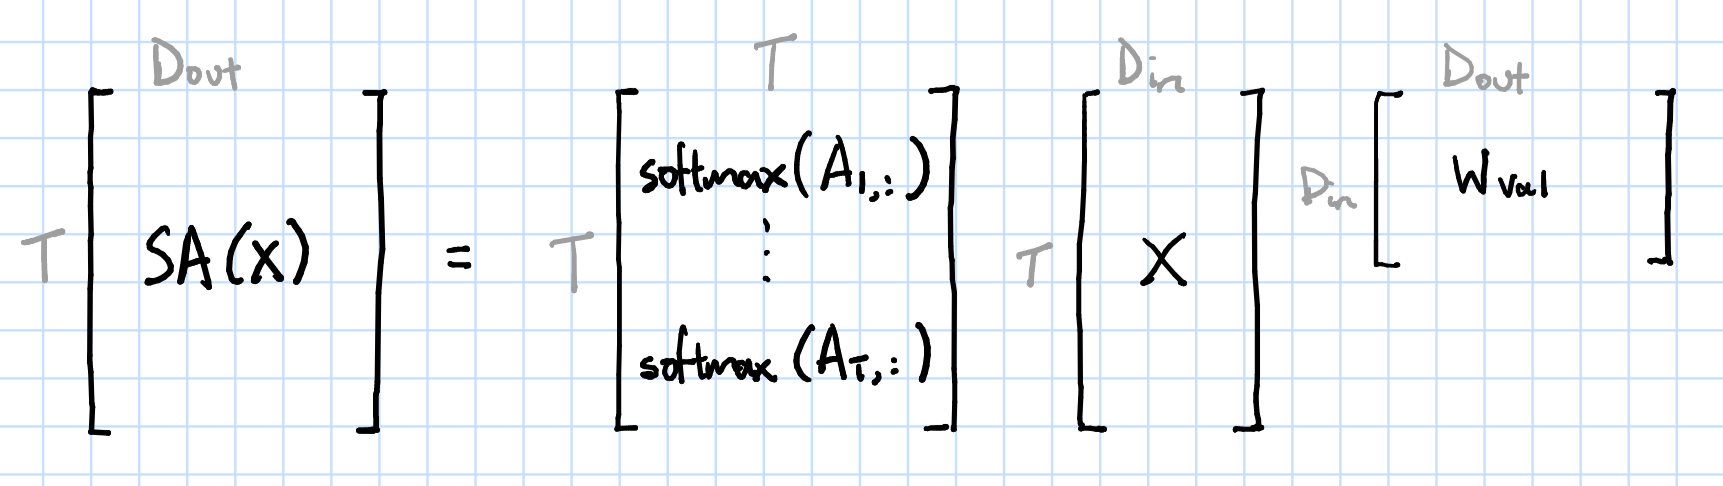
\includegraphics[width=.7\textwidth]{images/softmax.png}
\end{center}
\vspace{.1in}

\item We refer to the the elements of the $T\times T$ matrix
\begin{equation}
\mb A \doteq \mb X \mb W_{qry}\mb W_{key}^T\mb X^T
\end{equation}
the {\em attention scores}, and the softmax outputs as {\em attention probabilities}.
\end{itemize}
\end{frame}


\begin{frame}{Self-Attention}
\begin{itemize}
\item So far the learnable parameters are the {\em query}, {\em key}, and {\em value} matrices
$$\mb W_{qry} \in \bb R^{D_{in}\times{D_k}}, \ \ 
\mb W_{key} \in \bb R^{D_{in}\times{D_k}},\ \text{ and } \ 
\mb W_{val} \in \bb R^{D_{in}\times{D_{out}}}.$$
For simplicity, ignore residual connections, normalization or constant factors.

\vspace{.15in}
\item Note that $\bm A$ is {\em permutation equivariant} -- shuffling the order of the tokens (rows) in $\bm X$ shuffles the token scores in $\bm A$. {\em This is not desired behavior.}
\begin{itemize}
    \item e.g. "the cat ate the fish" is very different from "the fish ate the cat"
\end{itemize}

\vspace{.1in}
\item To overcome this, we can add a (fixed or learned) {\em positional encoding} $\bm P_{t,:}$, for each token in the sequence, to the input matrix for computing attention scores
\begin{equation}
A \doteq (\mb X + \mb P)\mb W_{qry}\mb W_{key}^T (\mb X + \mb P)^T,
\end{equation}
where the encoding matrix $\bm P$ has size $T\times D_{in}$.
\end{itemize}
\end{frame}


\newcommand{\WW}{ \mb W_{qry}\mb W_{key}^T }
\begin{frame}{Relative positional encoding}
\begin{itemize}
\item In {\em absolute encoding}, a fixed or learned vector $\bm P_{t,:}$ is assigned to each token $t$. Therefore, for a query token $q$ (the token to compute the representation of) and key token $k$ (the pixel we are attending to),
\begin{align}
    \mb A^{abs}_{q, k} 
        \ &=\ (\mb X_{q,:} + \mb P_{q,:})\WW(\mb X_{q,:} + \mb P_{q,:})^T 
        \nonumber
        \\ &=\ \mb X_{q,:}\WW\mb X^T_{k,:} +\ \mb X_{q,:}\WW\mb P^T_{k,:} 
        \\ &\qquad +\ \mb P_{q,:}\WW\mb X^T_{k,:} \ +\ \mb P_{q,:}\WW\mb P^T_{k,:} \nonumber 
\end{align}

\item \emph{Relative positional encoding} instead considers the positional difference between the query and key tokens:
\vspace{-.05in}
\begin{align}
    \mb A^{rel}_{q, k} &= 
        \mb X_{q,:}^T \WW \mb X_{k,:}
        + \mb X_{q,:}^T \mb W_{qry}^T\hat{\mb W}_{key} \mb r_{\delta}
        + \mb u^T \mb W_{key} \mb X^T_{k,:}
        + \mb v^T \hat{\mb W}_{key} \mb r_{\delta}.
    \label{relposenc}
\end{align}
\vspace{-.18in}
\begin{itemize}
    \item The learnable vectors $\bm u$, $\bm v$ are unique for each head 
    \item The relative positional encoding $\bm r_{\delta} \in \bb R^{D_p}$ depends only on the shift $\delta \doteq k -q$, and is shared by all layers and heads.
    \item Key weights are split into $\bm W_{key}$ for the input and $\hat{\bm W}_{key}$ for positional encoding.
\end{itemize}

\item The attention scores are now {\em translation equivariant} rather than permutation equivariant. This is the desired behavior for convolutional / vision tasks.
\end{itemize}
\end{frame}


\begin{frame}{Multi-Head Self-Attention (MHSA)}
\begin{itemize}
\item In practice it is beneficial to replicate the SA mechanism into multiple heads, by concatenating the output of $N_h$ heads of output dimension $D_h$ and projecting it to dimension $D_{out}$.
\begin{equation}
\mathrm{MHSA}(\mb X) \doteq \mathrm{hcat}_{h\in[N_h]}\big[\mathrm{SA}_h(\mb X)\big]\mb W_{out} + \mb b_{out}. \label{mhsa}
\end{equation}
Here $\bm W_{out}\in\bb R^{N_hD_h\times D_{out}}$ is the projection matrix and $\bm  b_{out}\in\bb R^{D_{out}}$ is a bias term.

\vspace{.2in}
\begin{center}
    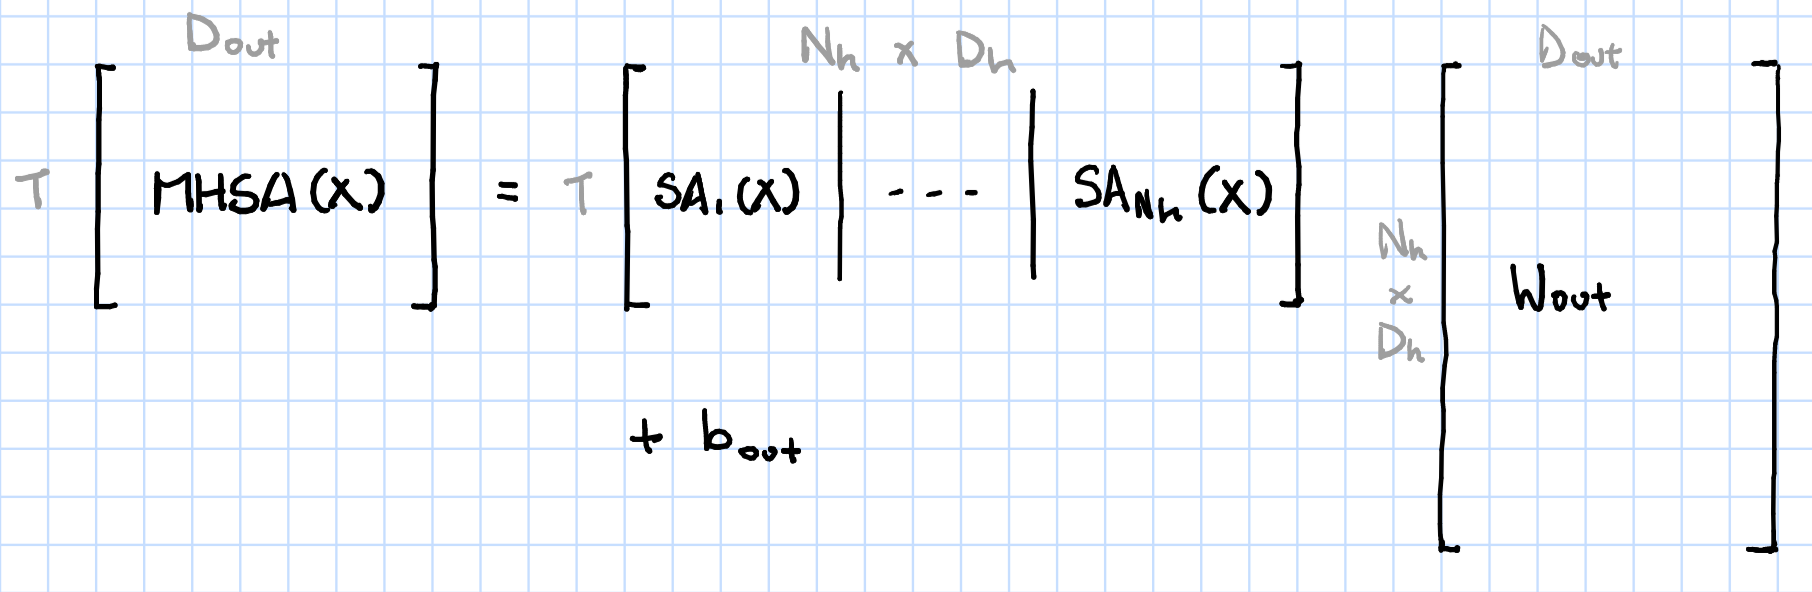
\includegraphics[width=.7\textwidth]{images/mhsa.png}
\end{center}
\end{itemize}
\end{frame}


\begin{frame}{Self-Attention for Images}
\framesubtitle{From 1D sequence to 2D}
\begin{itemize}
\item Replace query and key tokens with pixels $\bm q, \bm k \in [W]\times[H]$, and the input with $\bm X \in \bb R^{W\times H\times D}$. Each attention score now associates a query and key pixel. 

\item For a pixel $\bm p\in (i,j), \bm X_{\bm p,:} \doteq \bm X_{i,j,:}$ and $\bm A_{\bm p, :} \doteq \bm A_{i,j,:,:}$. 

\item Then, analogously to the 1D case,
\begin{equation}
\mathrm{SA}(\mb A)_{\mb q, :} \ = \ \sum_{\mb k} \mathrm{softmax}(\mb A_{\mb q, :})_{\mb k}\ \mb X_{\mb k, :} \ \mb W_{val},
\end{equation}
and relative positional encoding retains the same form as Equation \eqref{relposenc}. Similarly MHSA retains the same form as Equation \eqref{mhsa}.
\end{itemize}
\end{frame}


\newcommand{\sqbrkt}[1]{\left[#1\right]}
\newcommand{\ktwo}{\left\lfloor\frac K2\right\rfloor}
\begin{frame}{Self-Attention for Images}
\framesubtitle{Convolution}
\begin{itemize}
\item Given an image tensor $\bm X \in \bb R^{W\times H\times D_{in}}$ and kernel tensor $\bm W \in \bb R^{K\times K \times D_{in} \times D_{out}}$,
\begin{equation}
\mathrm{Conv}(\mb X)_{i,j,:} \ \doteq \ \sum_{(\delta_1, \delta_2) \in \Delta_K} \mb X_{i-\delta_1, j-\delta_2, :} \mb W_{\delta_1, \delta_2, :, :} + \mb b \ \ \in \ \mathbb R^{D_{out}},
\end{equation}
where
$$\Delta_K \ \doteq \ \sqbrkt{-\ktwo, \dots, \ktwo} \times \sqbrkt{-\ktwo, \dots, \ktwo}$$
is the set of all shifts represented by a $K\times K$ kernel.

\vspace{.1in}
\item We depart from the original notation slightly by using the {\em unflipped} convolution. In the paper, the summand is flipped to $\bm X_{i+\delta_1, i+\delta_2,:} \bm W_{\delta_1, \delta_2,:,:}$. The theorem in the paper is not changed by this.
\end{itemize}
\end{frame}


\begin{frame}{Self-Attention as a Convolutional Layer}
\framesubtitle{Main Theorem}
\begin{itemize}
\item \textbf{Main theorem.} \emph{A {\em multi-head self-attention} (MHSA) layer with $N_h$ heads of dimension $D_h$ each, final output dimension $D_{out}$, and a {\em relative positional encoding} of dimension $D_p\geq3$ can express any 2D convolutional layer of kernel size $\sqrt{N_h}\times\sqrt{N_h}$ and $\min(D_h, D_{out})$ output channels.}

\begin{center}
    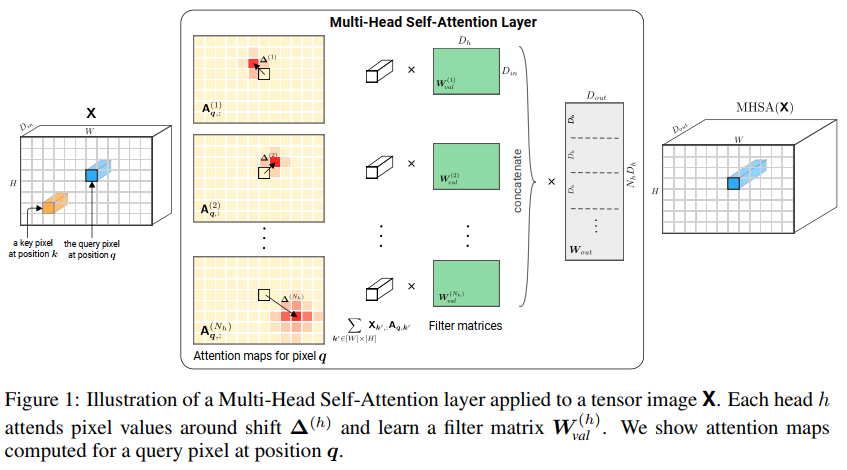
\includegraphics[width=.8\textwidth]{presentation/images/sa_as_conv.png}
\end{center}
\vspace{-.15in}

\item The theorem is a consequence of two lemmas.
\end{itemize}
\end{frame}


\begin{frame}{Self-Attention as a Convolutional Layer}
\framesubtitle{Lemma 1}
\begin{itemize}
\item \textbf{Lemma 1.} {\em Consider a MHSA layer consisting of $N_h = K^2$ heads, $D_h\geq D_{out}$ and let $\bm f:[N_h]\rightarrow\Delta_K$ be a bijective mapping of heads onto shifts. Further, suppose that for every head
\begin{equation}
\mathrm{softmax}(\mb A^{(h)}_{\mb q,:})_{\mb k} = \begin{cases}
    1 & \text{if } \mb f(h) = \mb q - \mb k,
    \\ 0 & \text{otherwise}.
    \end{cases} \label{lemma1_assumption}
\end{equation}
Then for any convolutional layer with a $K\times K$ kernel and $D_{out}$ output channels, there exists $\{\bm W_{val}^{(h)}\}_{h\in[N_h]}$ such that $\mathrm{MHSA}(\bm X) = \mathrm{Conv}(\bm X)$, for any kernel tensor $\bm W \in \bb R^{K\times K \times D_{in} \times D_{out}}$, and for all $\bm X\in\bb R^{W\times H\times D_{in}}$.}

\vspace{.05in}
\item \textit{Proof of Lemma 1.} Rewrite Equation \eqref{mhsa} as
\begin{equation}
    \mathrm{MHSA}(\mb X) = \mb b_{out} + 
        \sum_{h\in[N_h]} \mathrm{softmax}(\mb A^{(h)})\ \mb X\ 
        \underbrace{\mb W_{val}^{(h)}\ \mb W_{out}^{(h)}}_{\mb W^{(h)}}\ .
    \vspace{-.1in}
\end{equation}
Here $\bm W_{val}^{(h)} \in \bb R^{D_{in}\times D_h}$ is the value matrix for head $h$, or in MATLAB notation,
$$\bm W_{out}^{(h)} = \bm W[(h-1)*D_h+1 : hD_h\ , \ :\ ] \ \ \in\ \ \bb R^{D_h\times D_{out}}.$$
\end{itemize}
\end{frame}


\newcommand{\row}[1]{_{#1,:}}
\begin{frame}{Self-Attention as a Convolutional Layer}
\framesubtitle{Lemma 1}
\begin{itemize}
\item \textit{Proof of Lemma 1 (cont).} Consider a single "query" pixel from $\mathrm{MHSA}(\bm X)$:
\begin{equation}
    \mathrm{MHSA}(\mb X)\row {\mb q} = \mb b_{out} + 
        \sum_{h\in[N_h]} \left( \sum_{\mb k\in [T]} 
            \mathrm{softmax}(\mb A^{(h)}\row {\mb q})_{\mb k}\ \mb X\row{\mb k} 
        \right) \mb W^{(h)} .
\end{equation}
The summand $\sum_{\mb k} \mathrm{softmax}(\mb A^{(h)}\row {\mb q})_{\mb k}\ \mb X\row{\mb k}$ is a weighted average on the rows of $\bm X$. 

\item Applying the assumption from Equation \eqref{lemma1_assumption}, each of the softmax weights pick out a single row $\bm k = \bm q - \bm f(h)$:
\begin{equation}
    \mathrm{MHSA}(\mb X)\row {\mb q} = \mb b_{out} + 
        \sum_{h\in[N_h]}  \mb X\row{\mb q - \mb f(h)} \mb W^{(h)} .
\end{equation}

If we set $K=\sqrt{N_h}$, then it is clearly possible to index all the shifts using $h\in[N_h]$, i.e. $\bm f([N_h]) = \Delta_K$. Therefore we can rewrite the expression as
\begin{equation}
    \mathrm{MHSA}(\mb X)\row {\mb q} = \mb b_{out} + 
        \sum_{h\in[N_h]}  \mb X\row{\mb q - \mb f(h)} \mb W_{\mb f(h), :, :} 
        = \mathrm{Conv}(\mb X)\row{\mb q}. 
    \quad\qed
\end{equation}
\end{itemize}
\end{frame}


\begin{frame}{Self-Attention as a Convolutional Layer}
\framesubtitle{Lemma 1}
\begin{itemize}
\item Lemma 1 says that, with the right choice of relative positional encoding (and a very restricted set of attention parameters), {\em a MHSA layer is exactly equivalent to a convolutional layer}.

\vspace{.1in}
\item The number of linearly independent filters expressible by $\bm W$ is clearly limited by $\min(D_h, D_{out})$. Therefore, to express $D_h$ convolutional filters, it is best to simply let $D_{out} = N_hD_h$ and have $\bm W^{(h)}\in\bb R^{D_h\times D_h}$. 

\vspace{.1in}
\item There is a generalized version of this lemma in the Appendix of the paper that delves into the space of filters spannable for a given set of dimensions $D_h, N_h, D_{out}$, etc., for interested readers.
\end{itemize}
\end{frame}


\newcommand{\brac}[1]{^{(#1)}}
\begin{frame}{Self-Attention as a Convolutional Layer}
\framesubtitle{Lemma 2}
\begin{itemize}
\item \textbf{Lemma 2.} {\em There exists a relative encoding scheme $\{\bm r_{\bm \delta} \in \bb R^{D_p}\}_{\bm \delta\in\bb Z^2}$ with $D_p\geq 3$ and parameters $\bm W_{qry}$, $\bm W_{key}$, $\hat{\bm X}_{key}$, $\bm u$ with $D_p\leq D_k$ such that, for every $\bm\varDelta \in \Delta_K$ there exists some vector $\bm v(\bm\varDelta)$ that yields $\mathrm{softmax}(\bm A_{\bm q,:})_{\bm k}=1$ if $\bm k - \bm q = \bm\varDelta$, and zero otherwise.}

\vspace{.1in}
\item \textit{Proof of Lemma 2.} Start with the relative positional encoding of Equation \eqref{relposenc}:
\begin{equation*}
    \mb A^{rel}_{\mb q, \mb k} = 
        \mb X_{\mb q,:}^T \WW \mb X_{k,:}
        + \mb X_{\mb q,:}^T \mb W_{qry}^T\hat{\mb W}_{key} \mb r_{\mb \delta}
        + \mb u^T \mb W_{key} \mb X^T_{k,:}
        + \mb v^T \hat{\mb W}_{key} \mb r_{\bm\delta}.
\end{equation*}
Since the desired attention probabilities \eqref{lemma1_assumption} from Lemma 1 are independent of the input $\bm X$, set $\bm W_{key}=\bm W_{qry} = \bm 0$. 

\vspace{.1in}
This leaves only the final term. Setting $\hat{\bm W}_{key} = [\ \bm I_{D_p}\ ; \ \bm 0\ ] \in \mathbb R^{D_k\times D_p}$ (recall $D_p\leq D_k$) yields
\begin{equation*}
    \mb A_{\mb q, \mb k} = \mb v_{1:D_p}^T\, \mb r_{\bm\delta}.
\end{equation*}
\end{itemize}
\end{frame}


\newcommand{\sqnorm}[1]{\Vert#1\Vert^2}
\newcommand{\expalpha}[1]{e^{-\alpha#1}}
\newcommand{\limalpha}{\lim_{\alpha\rightarrow\infty}}
\newcommand{\vDelta}{\varDelta}
\begin{frame}{Self-Attention as a Convolutional Layer}
\framesubtitle{Lemma 2}
\begin{itemize}
\item \textit{Proof of Lemma 2 (cont).} Recall that $\bm \delta \doteq \bm k - \bm q$. Now suppose some $\bm v, \bm r_{\bm \delta}$ could be found such that
\begin{equation}
    \mb A_{\mb q, \mb k} = -\alpha(\sqnorm{\bm{\delta - \varDelta}} + c) 
    \label{lemma2_attnreq}
\end{equation}
so that the maximum score $-\alpha c$ is achieved when $\bm\delta = \bm\varDelta$, then
\begin{align*}
    \limalpha \text{softmax}(\mb A_{\mb q, :})_{\mb k} &\eq 
        \limalpha\frac{\expalpha{(\sqnorm{\bm{\delta-\varDelta}}+c)}}{
            \sum_{\bm\delta'\in\Delta_K}
            \expalpha{(\sqnorm{\bm{\delta'-\varDelta}}+c)}
        } \\ &\eq \frac{1_{\bm\delta=\bm\varDelta}}{
            1 + \limalpha\sum_{\bm\delta'\neq \bm\delta}
            \expalpha{\sqnorm{\bm{\delta'-\varDelta}}}
        } = 1_{\bm\delta=\bm\varDelta}.
\end{align*}

\item Choosing $\bm v_{1:D_p} = -\alpha(1, -2\varDelta_1, -2\varDelta_2)$ and $\bm r_{\bm \delta} = (\Vert\bm \delta\Vert^2, \delta_1, \delta_2)$, yields
\begin{align*}
    \mb A_{\mb q, \bm k} &= 
        \mb v_{1:D_p}^T\, \mb r_{\bm \delta}
        \\ &= -\alpha(\sqnorm{\bm\delta} -2\vDelta_1\delta_1-2\vDelta_2\delta_2) 
        \\ &= -\alpha(\sqnorm{\bm\delta-\bm\vDelta} - \sqnorm{\bm\vDelta}).
\end{align*}
Setting $c=-\sqnorm{\bm\varDelta}$ recovers Equation \eqref{lemma2_attnreq} and completes the proof. \qed
\end{itemize}
\end{frame}


\begin{frame}{Self-Attention as a Convolutional Layer}
\framesubtitle{Lemma 2}
\begin{itemize}
\item The encoding scheme satisfying Lemma 2 is a {\em quadratic encoding scheme}, and is achieved by setting
\begin{align}
    \mb v\brac h &\doteq -\alpha\brac h 
        (1, -2\varDelta_1\brac h, -2\varDelta_2\brac h), \nonumber \\
    \mb r_{\bm \delta} &\doteq (\Vert\bm\delta\Vert^2,\ \delta_1,\ \delta_2), 
    \label{quad_encoding} \\
    \mb W_{qry} &= \mb W_{key} \doteq \bm 0, \nonumber \\
    \hat{\mb W}_{key} &\doteq \mb I. \nonumber
\end{align}
Here the learned parameters $\bm\varDelta^{(h)} = (\varDelta_1^{(h)}, \varDelta_2^{(h)})$ and $\alpha^{(h)}$ determine the center and width of attention of each head, and $\bm\delta = (\delta_1, \delta_2)$ is fixed and expresses the relative shift between query and key pixels.

\item Although the proof requires $\alpha\rightarrow\infty$ to satisfy the assumption \eqref{lemma1_assumption} of Lemma 1, finite precision arithmetic performs hard attention with sufficiently large enough $\alpha$. E.g. for \texttt{Float32}, set $\alpha\geq46$. 

\item The lemma, and thus the theorem, can be extended in a straightforward manner to cover $K$-dimensional convolutions, with $D_p=K+1$.
\end{itemize}
\end{frame}


\begin{frame}{Experimental Setup}
\begin{itemize}
\item \textbf{Baseline.} Standard ResNet18 on CIFAR-10

\vspace{.02in}
\item \textbf{Model.}
\begin{itemize}
    \item 6 MHSA layers. Each layer consists of a MHSA step, followed by dense, dropout and LayerNorm sublayers.
    \item Use 2x2 invertible downsampling to reduce image size (attention coefficients scale quadratically to image size)
    \item Fixed size representation of input image is the average pooling of the last layer representations, and fed to a linear classifier
\end{itemize}

\vspace{.02in}
\item \textbf{MHSA variations.} Different types of relative positional encoding
\begin{equation*}
    \mb A^{rel}_{\mb q, \mb k} = 
        \mb X_{\mb q,:}^T \WW \mb X_{k,:}
        + \mb X_{\mb q,:}^T \mb W_{qry}^T\hat{\mb W}_{key} \mb r_{\mb \delta}
        + \mb u^T \mb W_{key} \mb X^T_{k,:}
        + \mb v^T \hat{\mb W}_{key} \mb r_{\bm\delta}.
    \vspace{-.12in}
\end{equation*}
\begin{itemize}
    \item \textbf{SA with quadratic embedding:}  Retain final term only and fix the variables using Equation \eqref{quad_encoding}. The attention widths $\alpha^{(h)}$ and centers $\varDelta^{(h)}$ are still learnt.
    \item \textbf{SA with learned embedding:} Retain final term only but learn $\mathbf v,\ \hat{\mathbf W}_{key},\ \mathbf r_{\bm \delta}$, with $D_p=D_{out}=400$. Set $D_h=D_{out}$.
    \item \textbf{SA with content-based attention:} All terms retained (might actually be just first two terms) and all variables learnable. Same dimensions as above.
\end{itemize}
\end{itemize}
\end{frame}


\begin{frame}{Convergence / Testing Accuracy}
\begin{columns}
\begin{column}{0.43\textwidth}
  \begin{itemize}
    \item \textbf{ResNet converges faster:} Probably because SA's inductive bias is not as strong as ResNet, but may also be due to different optimization setup.
    
    \vspace{.1in}
    \item SA models with more learnable parameters converge slower and ends up with lower testing accuracy.  
  \end{itemize}
\end{column}
\begin{column}{0.55\textwidth} \centering
  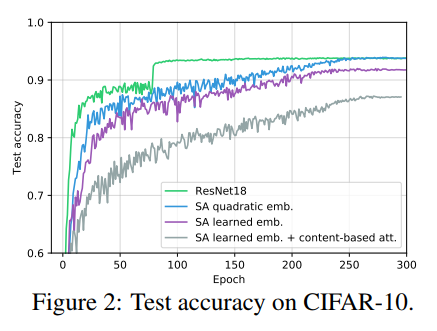
\includegraphics[width=\textwidth]{presentation/images/converge_test_acc.png}
\end{column}
\end{columns}
\end{frame}


\begin{frame}{Do Self-Attention Layers Actually Learn Convolutions? Maybe.}
\begin{itemize}
\item Recall that from Lemma 1, the critical assumption is
\begin{equation*}
    \mathrm{softmax}(\mb A^{(h)}_{\mb q,:})_{\mb k} 
        = \bm 1_{\bm f(h) = \bm q - \bm k}, 
        \quad \forall h.
\end{equation*}
If $N_h=\abs{\Delta_K}$, mapping each head to a single shift $\bm f(h)=\bm\varDelta\in\Delta_K$ yields 
\begin{equation*}
    \mathrm{softmax}(\mb A^{\bm\varDelta}_{\mb q,:})_{\mb k} 
        = \bm 1_{\bm \varDelta = \bm q - \bm k}, 
        \quad \forall \bm\varDelta.
\end{equation*}

\item MHSA expresses a single convolution operation when attention probabilities are all elements of a {\em translation group}. For instance, this would also suffice:
\begin{equation*}
    \mathrm{softmax}(\mb A^{\bm\varDelta}_{\mb q,:})_{\mb k} 
        = \tfrac1\tau\ \bm 1_{\abs{\bm \varDelta - (\bm q - \bm k)}\leq\tau},
        \quad \forall \bm\varDelta.
\end{equation*}

\item Alternatively, if we remove some of the shifts from $\Delta_K$, the heads are still elements of a translation group and we just end up with {\em sparse} convolution.

\item And if there were multiple distribution profiles in the attention probabilities, then MHSA can be seen as expressing a {\em mixture} of convolution operators.

\item \textbf{Takeaway:} \emph{It's difficult to judge whether a MHSA layer has a preference for learning convolutional operators or not, especially when $N_h$ is small.}
\end{itemize}
\end{frame}


\begin{frame}{Do Self-Attention Layers Actually Learn Convolutions? Maybe.}
\framesubtitle{Quadratic encoding}
\begin{itemize}
\item $N_h=9$ heads
\begin{center}
    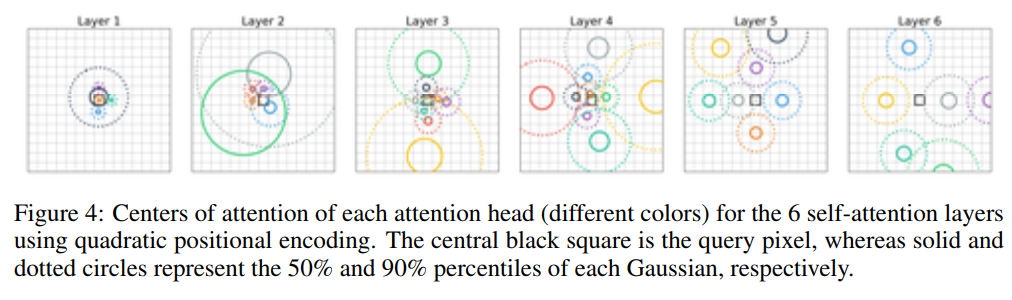
\includegraphics[width=.75\textwidth]{presentation/images/quad_emb_9.png}
\end{center}

\item $N_h=16$ heads
\begin{center}
    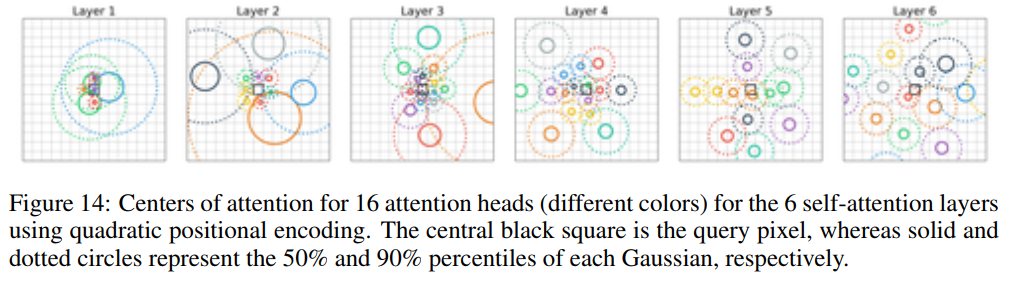
\includegraphics[width=.75\textwidth]{presentation/images/quad_emb_16.png}
\end{center}

\end{itemize}
\end{frame}


\begin{frame}{Do Self-Attention Layers Actually Learn Convolutions? Maybe.}
\framesubtitle{Learned relative positional encoding (w/o content)}
\begin{center}
    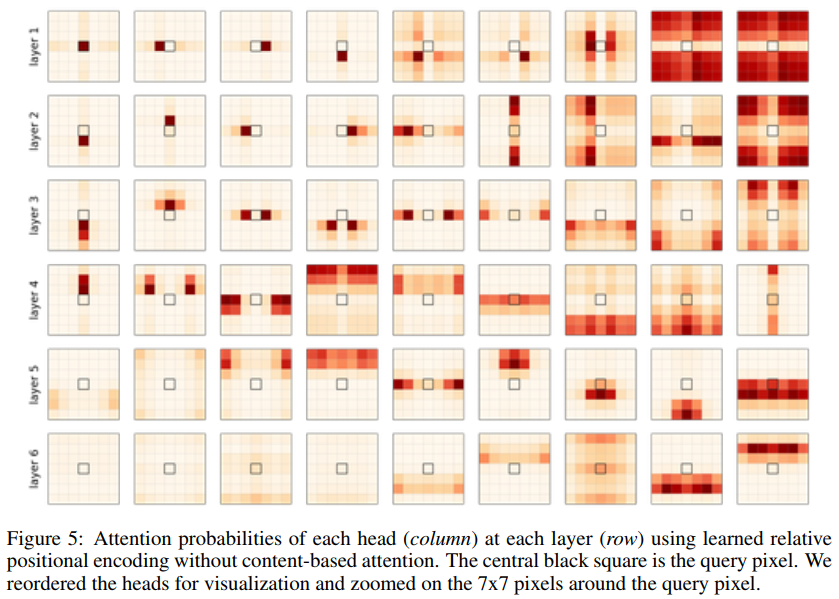
\includegraphics[width=.7\textwidth]{
        presentation/images/learned_rel_emb_nocontent.png}
    \vspace{-.1in}
\end{center}
\begin{itemize}
\item Each layer seems to mostly learn one or two attention profiles. 
\end{itemize}
\end{frame}


\begin{frame}{Do Self-Attention Layers Actually Learn Convolutions? Maybe.}
\framesubtitle{Learned relative positional encoding with content}
\begin{center}
    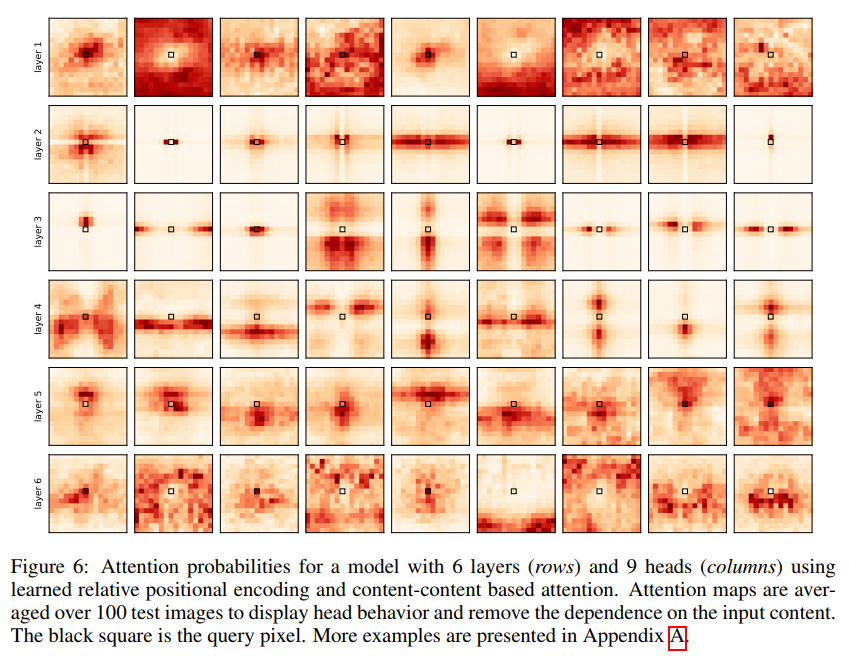
\includegraphics[width=.68\textwidth]{
        presentation/images/learned_rel_emb_content.png}
    \vspace{-.1in}
\end{center}
\begin{itemize}
\item Still demonstrates some of the behavior shown for the learned embeddings without content.
\end{itemize}
\end{frame}


% Final slide
\usebackgroundtemplate{ %       declare background
\tikz[overlay,remember picture] \node[opacity=1, at=(current page.center)] {
   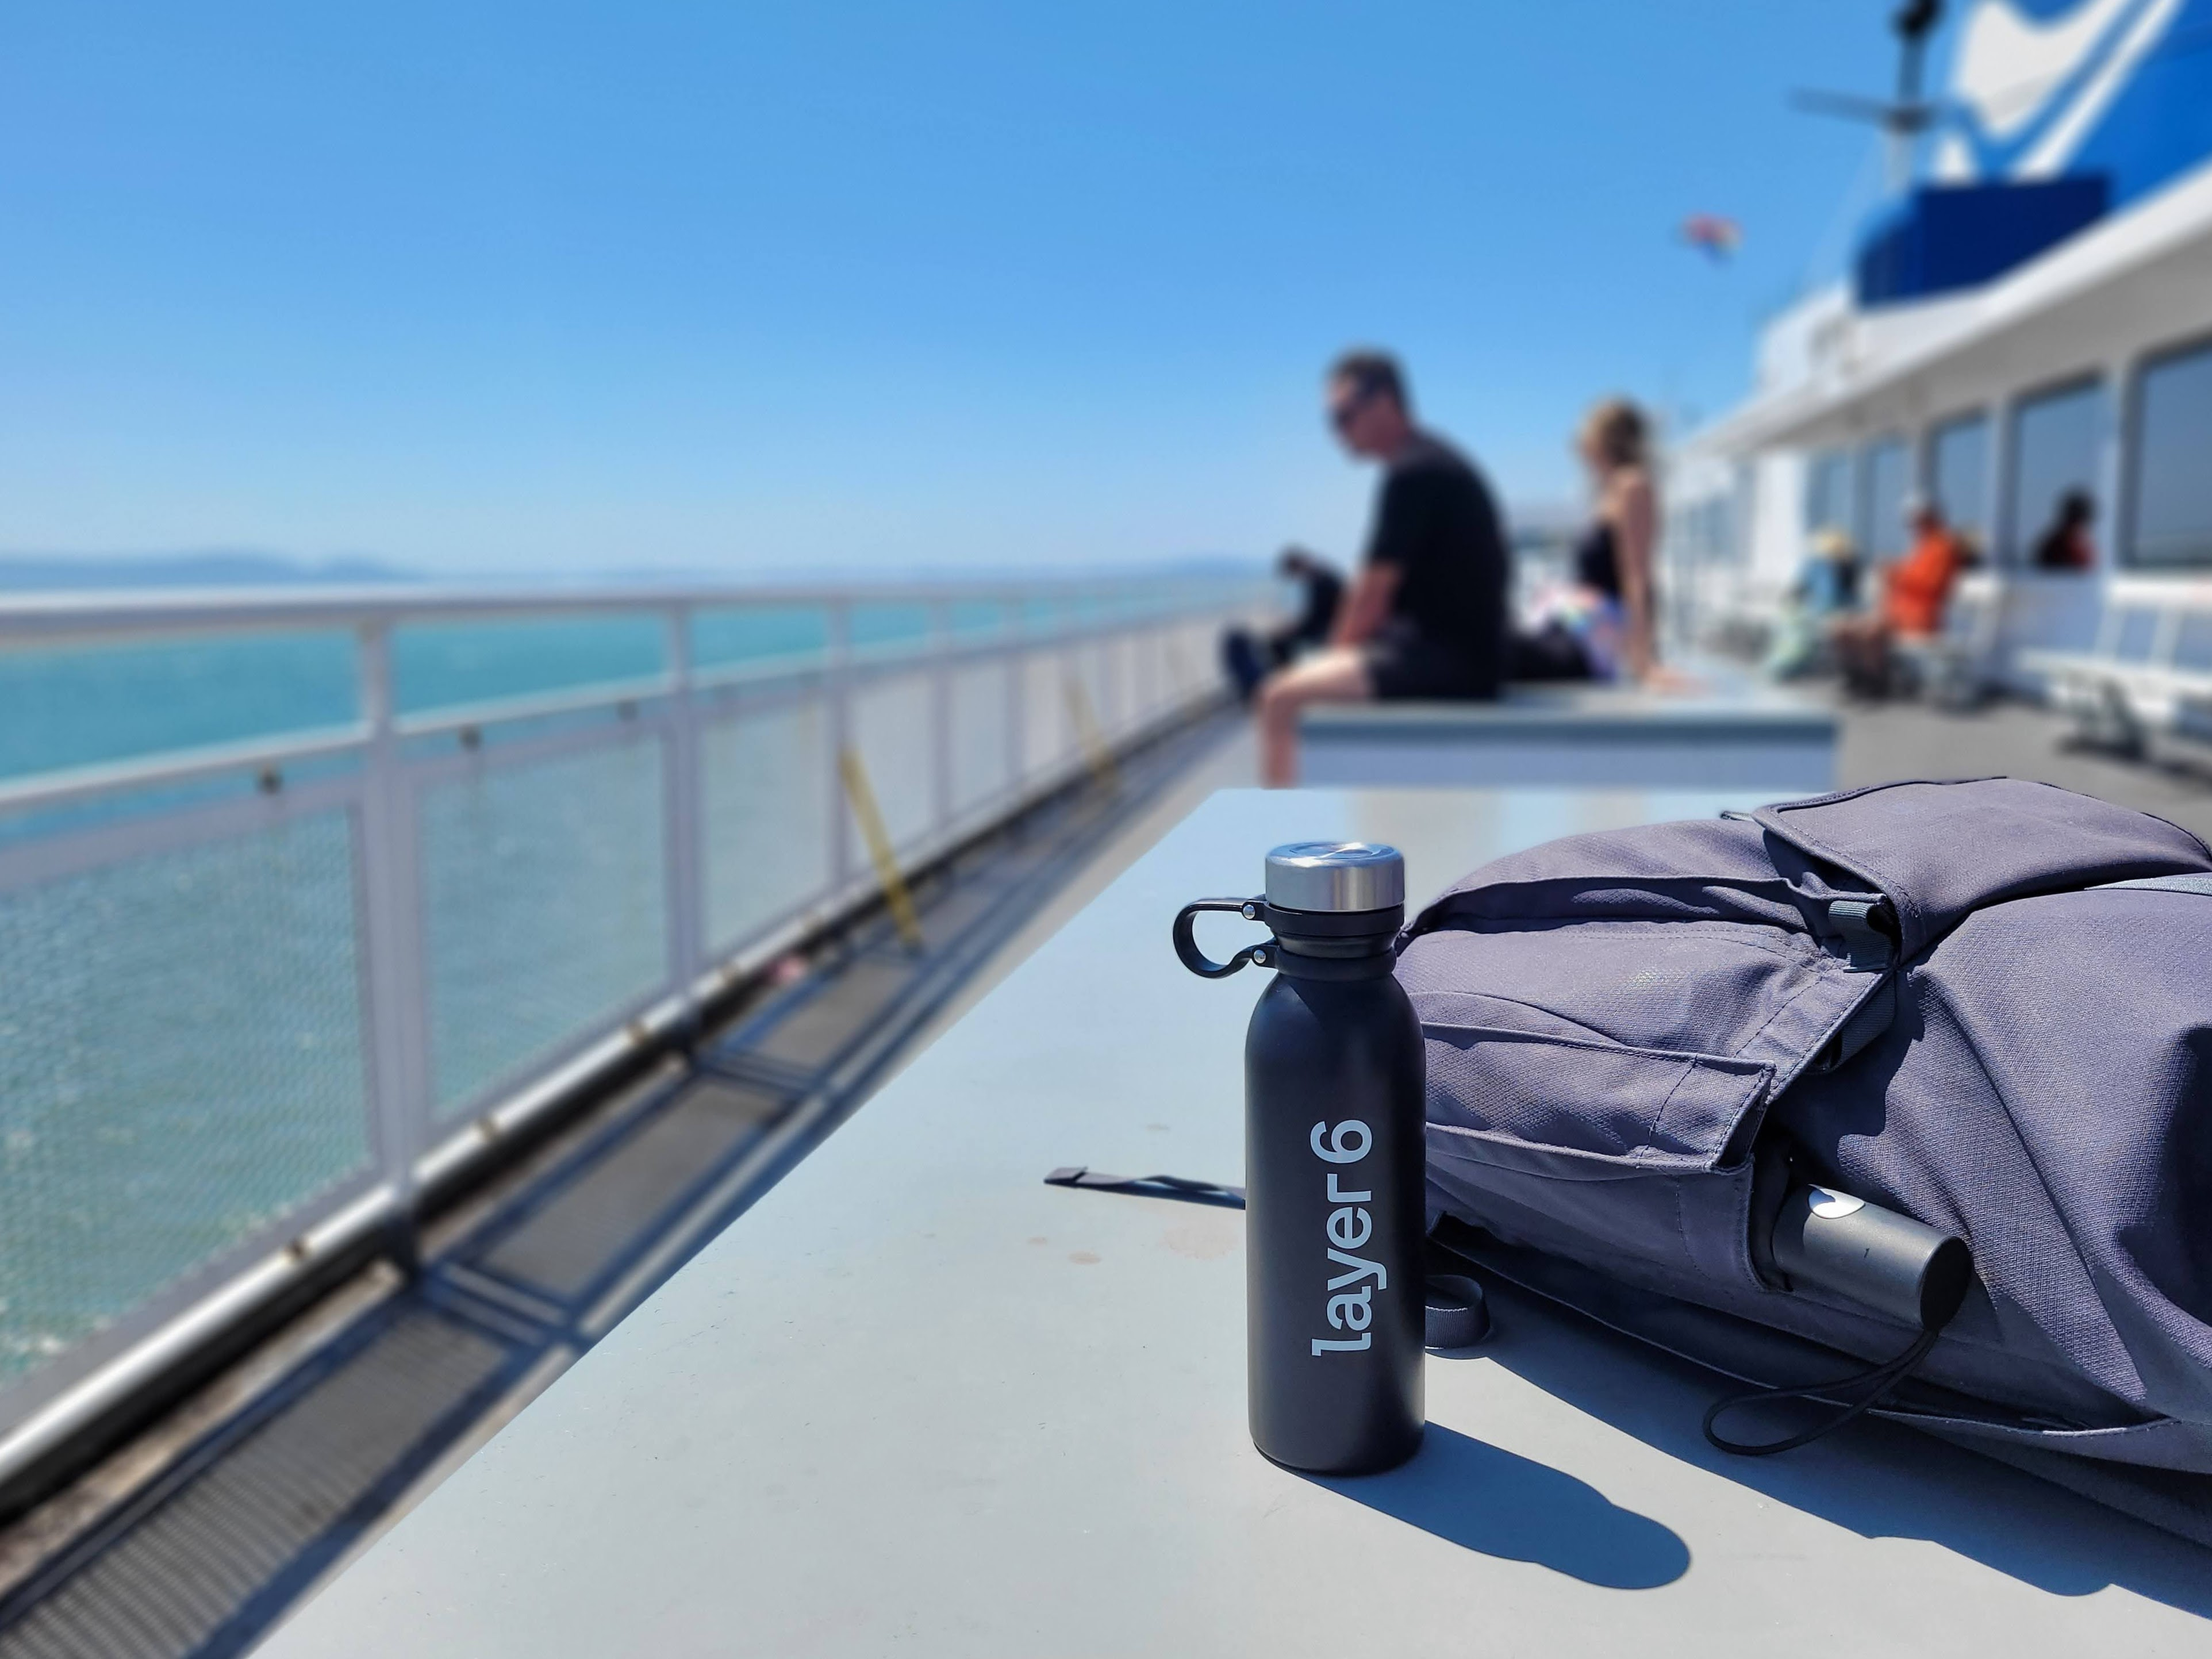
\includegraphics[height=\paperheight,width=\paperwidth]{presentation/images/l6_bottle_bc_1.jpg}};
}
\begin{frame}
\begin{textblock}{8}(1.8, 4.2) \raggedright \Huge 
    Thanks for listening!
\end{textblock}
\end{frame}
\usebackgroundtemplate{ } %%    undeclare background

\end{document}